\chapter{Dasar Teori}
\label{chap:dasar_teori}
Pada bab ini akan dijelaskan dasar-dasar teori mengenai Android SDK, Google VR SDK,Quaternion, \textit{Sensor Fusion}, dan algoritma \textit{Head Motion Detection}.

\section{Android SDK}
\label{sec:android_sdk}

Android SDK(\textit{software development kit}) adalah kumpulan \textit{source code, development tools, emulator,}\cite{developers2011android} dan semua \textit{libraries} untuk membuat suatu aplikasi untuk \textit{platform} Android. IDE(\textit{integrated development environment} yang official untuk Android SDK adalah Android Studio. Android Studio dapat di download di halaman website \url{https://developer.android.com/studio/index.html}, sekaligus dengan Android SDKnya. 
\subsection{Membuat Android \textit{Project}}
Pada bagian ini akan ditunjukkan bagaimana membuat Android Project baru dengan Android Studio.
\begin{enumerate}
	\item Membuah suatu \textit{project} baru di android studio dengan memilih \textbf{File \textgreater New Project}
	\item Kemudian isilah \textbf{Application Name} dan \textbf{Company Domain} pada halaman \textbf{New Project} sesuai dengan keinginan seperti yang ditunjukkan pada Gambar \ref{fig:android-studio-create-new-project}.
	Android studio akan mengisikan lokasi project dan nama package secara otomatis. 
	\item Klik \textbf{Next}
	\item Pada halaman \textbf{Target Android Devices}, klik \textbf{Next}.
	\item Pada halaman \textbf{Add an Activity to Mobile}, pilih \textbf{Empty Activity} kemudian klik \textbf{Next}.
	\item Pada halaman \textbf{Target Android Devices}, klik \textbf{Next}.
	\item Pada halaman \textbf{Customize the Activity}, klik \textbf{Finish}.
\end{enumerate}
\begin{figure}[htbp]
	\centering
		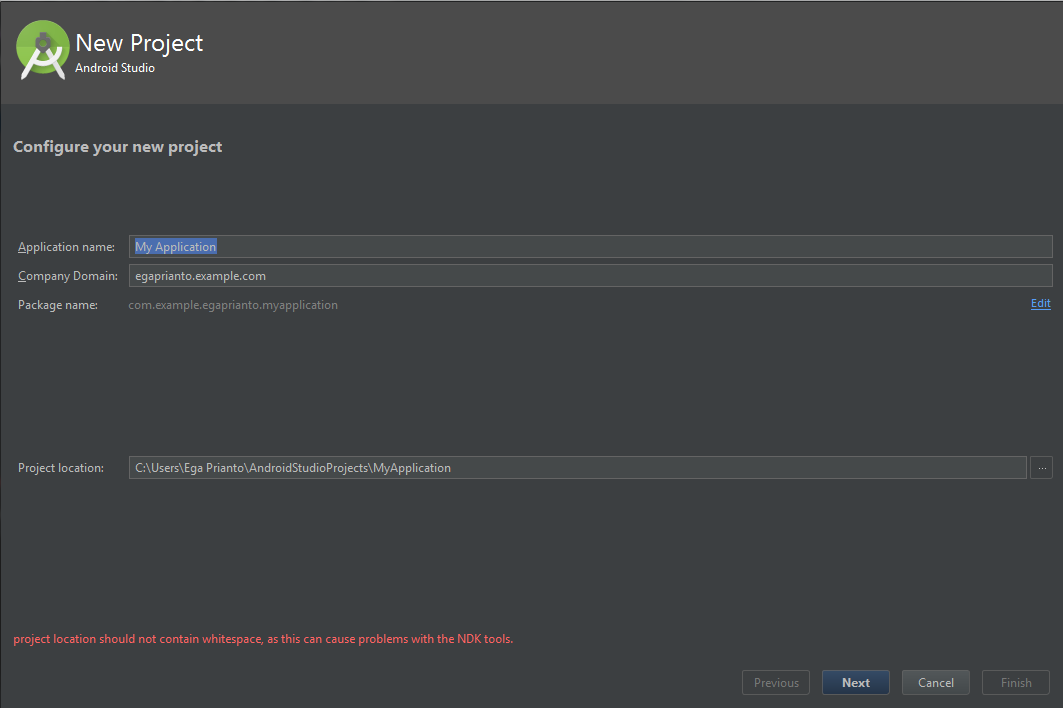
\includegraphics[scale=0.56]{Gambar/android-studio-create-new-project.png}
	\caption{Tampilan ketika membuat suatu \textit{project} baru}
	\label{fig:android-studio-create-new-project}
\end{figure}

Setelah diproses, Android Studio akan menampilkan aplikasi android dengan tulisan "`Hello Wold"'. 
\subsection{Struktur File Android Studio Project}
Pada saat \textbf{project} baru telah dibuat, Android Studio akan membuatkan direktori-direktori standar(Gambar \ref{fig:android-studio-structure}). Berikut adalah sebagian penjelasan dari hal yang perlu di perhatikan pada struktur tersebut:
\begin{enumerate}
	\item File \textbf{app\textgreater java\textgreater com.example.myfirstapp\textgreater MainActivity.java} mengandung definisi kelas untuk Activity Utama.
	\item File \textbf{app\textgreater res\textgreater layout\textgreater activity\_main.xml} adalah XML file untuk mendefinisikan\textit{layout}(\textit{User Interface}) dari suatu activity.
	\item File \textbf{app\textgreater manifests\textgreater AndroidManifest.xml} mendeskripsikan karakteristik fundamental dari suatu aplikasi dan juga mendefinisikan setiap komponennya.
	\item \textbf{Gradle Scripts\textgreater build.gradle}
	Android Studio menggunakan Gradle untuk melakukan \textit{compile} dan \textit{build} aplikasi Android. Pasti ada file build.gradle pada modul dan pada keseluruhan \textit{project}.
	\item Folder \textbf{res} 
	merupakan tempat untuk menyimpan sumber-sumber aplikasi seperti layout, icon, gambar, nilai konstan, dan lain-lain.
\end{enumerate}
\begin{figure}[htbp]
	\centering
		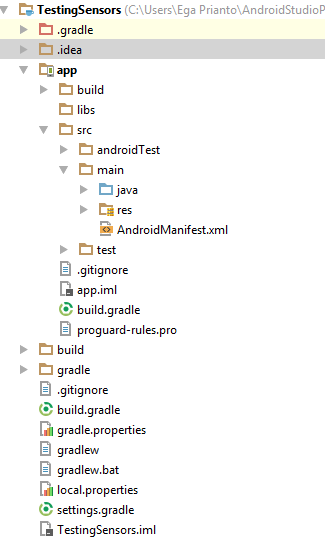
\includegraphics[scale=1]{Gambar/android-studio-structure.png}
	\caption{Tampilan struktur direktori pada \textit{project} Android Studio}
	\label{fig:android-studio-structure}
\end{figure}

\subsection{Membuat User Interface}
Pada subbab ini akan dijelaskan bagaimana membuat layout di XML termasuk \textit{text field} dan \textit{button}
\subsubsection{Hierarki \textit{Graphical User Interface}(GUI) untuk Aplikasi Android}
GUI untuk aplikasi Android dibuat dengan hierarki dari objek View dan ViewGroup(Gambar \ref{fig:viewgroup}). Objek-objek dari View biasanya adalah \textit{UI Widgets} seperti \textit{button} atau \textit{text field}. Objek-objek dari ViewGroup tidak terlihat oleh \textit{view containers} yang mendefinisikan bagaimana \textit{child views} ditata seperti \textit{grid} atau \textit{vertical list}
\begin{figure}[htbp]
	\centering
		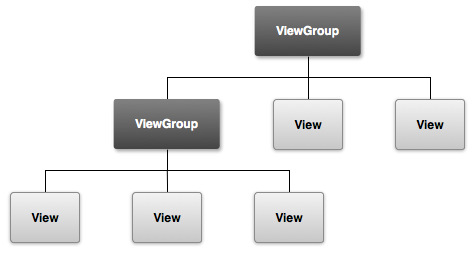
\includegraphics[scale=1]{Gambar/viewgroup.png}
	\caption{Illustrasi bagaimana percabangan objek ViewGroup pada \textit{layout} dan mengandung objek View lainnya.}
	\label{fig:viewgroup}
\end{figure}
Android menggunakan XML vocabulary yang berkorespondesi kepada \textit{subclasses} dari View dan ViewGroup, sehingga Ui dapat didefinisikan dalam XML menggunakan hierarki dari elemen UI.
\subsubsection{Attribut-attribut Objek View}
Pada subbab ini akan dijelaskan attribut-attribut object View yang digunakan dalam membuat GUI pada file activity\_main.xml
\begin{itemize}
	\item \textbf{android:id}
	Attribut ini merupakan pengidentifikasi dari suatu view. Attribut ini dapat digunakan untuk menjadi referrensi object dari kode aplikasi seperti membaca dan memanipulasi objek tersebut (Akan dijelaskan lebih lanjut pada subbab \ref{}). Tanda \textit{at} dibutuhkan ketika mereferensi object dari suatu XML. Tanda \textit{at} tersebut diikuti dengan tipe(id pada kasus ini), \textit{slash}, dan nama (edit\_message pada Gambar \ref{fig:attribute-view}). Tanda tambah (+) sebelum tipe hanya dibutuhkan jika ingin mendefinisikan \textit{resource ID} untuk pertama kalinya.
	\item \textbf{android:layout\_width} dan \textbf{android:layout\_height}
	Attribut ini digunakan untuk mendefinisikan panjang dan lebar dari suatu objek View. Daripada menggunakan besar spesifik untuk panjang dan lebarnya, lebih baik menggunakan "`wrap\_content"' yang menspesifikasi viewnya hanya akan sebesar yang dibutuhkan untuk memuat konten-konten dari View. Jika menggunakan "`match\_parent"' pada kasus Gambar \ref{fig:attribute-view} View akan memenuhi layar, karena besarnya akan mengikuti besar dari paretnya LinearLayout.
	\item \textbf{android:hint}
	Attribut ini merupakan \textit{default string} untuk di tampilkan ketika objek View kosong. Daripada menggunakan \textit{hard-coded string} sebagai \textit{nilai} untuk ditampilkan, \textit{value} "`@string/edit\_message"' mereferensi ke sumber string pada file yang berbeda. Karena mereferensi ke sumber konkrit, maka tidak dibutuhkan tanda tambah (+). Nilai string ini akan di simpan pada file Strings.xml yang ditunjukkan pada Gambar \ref{fig:android-studio-structure}.
	\item \textbf{android:onClick}
	Attribut ini akan memberitahu \textit{system} untuk memanggil method sendMessage() di Activity ketika user melakukan klik pada \textit{button} tersebut. Agar \textit{system} dapat memanggil method yang tepat, method tersebut harus memenuhi kriteria berikut.
	\begin{itemize}
		\item \textit{Access Modifier} haruslah \textit{public}.
		\item Harus \textit{void return value}nya.
		\item Mempunyai View sebagai parameter satu-satunya. View ini akan diisi dengan View yang di klik.
	\end{itemize}

\end{itemize}
\begin{figure}[htbp]
	\centering
		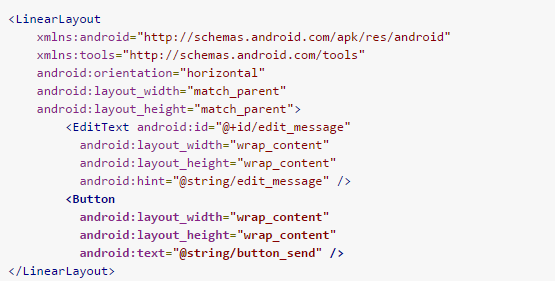
\includegraphics[scale=1]{Gambar/attribute-view.png}
	\caption{Contoh attribute pada objek View}
	\label{fig:attribute-view}
\end{figure}

 
\section{Google VR SDK}
\label{sec:google_vr_sdk}
\section{Quaternion}
\label{sec:quaternion}
Pada Android SDK \textbf{SensorEvent.values} \cite{android_developers} tipe sensor \textbf{Sensor.TYPE\_ROTATION\_VECTOR}, yaitu tipe sensor yang mendeteksi vektor perputaran pada \textit{smartphone}. Tipe sensor ini dijelaskan akan mengembalikan nilai-nilai dari komponen quaternion. 
Quaternion\cite{kuipers:1999} adalah objek penggabungan dari suatu skalar dengan suatu vektor, sesuatu yang tidak dapat didefinisikan dalam \textit{linear algebra} biasa. 
\subsection{Struktur Ajabar}
Struktur-Struktur aljabar yang digunakan adalah Bilangan Kompleks, Konjugasi Kompleks, \textit{Quaternion Algebra}, dan Operasi-operasi pada \textit{Quaternion}.
\subsubsection{Bilangan Kompleks}

Dalam matematika, bilangan kompleks adalah bilangan yang berbentuk\\
\[
	a+bi
\]\cite{kuipers:1999}\\
dan \(a\) dengan \(b\) merupakan bilangan riil, dan \(i\) merupakan bilangan imajiner tertentu yang memiliki sifat \(i^2=-1\).

Berikut notasi-notasi bilangan kompleks :
\[
 (a + bi) + (c + di) = (a+c) + i(b+d)
\]
\[
 (a + bi)(c + di) = (ac−bd) + (bc+ad)i
\]
\[
 a(c + id) = ac + iad
\]\cite{kuipers:1999}

Bilangan kompleks dapat digunakan untuk rotasi dua dimensi. Dengan \(a = \cos (\frac{\theta}{2})\), dan \(b = \sin(\frac{\theta}{2})\), kemudian akan dikalikan dengan vektor yang ingin di putar, dengan sumbu putar adalah titik pusat.


\subsubsection{Konjugasi Kompleks}
Berhubungan dengan bentuk umum bilangan kompleks,
\[
	z = a + ib
\]\cite{kuipers:1999}\\
satu bilangan dikatakan konjugasi kompleks jika
\[
	\bar{z} = a - ib
\]\cite{kuipers:1999}\\
Dari kedua persamaan diatas dapat dihasilkan :
\[
	z + \bar{z} = 2a
\]dan,
\[
	z \bar(z) = a^2 +b^2 = |z|^2
\]\cite{kuipers:1999}

\subsection{\textit{Quaternion Algebra} dan Operasi-operasi pada \textit{Quaternion}}
Pada buku "Quaternions and Rotation Sequences : A Primer with Applications to Orbits, Aerospace, and Virtual Reality" disebutkan :
\begin{quote}
In 1843 Hamilton invented the so-called hyper-complex number of rank 4, to which he gave the name \textit{quaternion}. Crucial to this invention was his celebrated rule
\[
	i^2 = j^2 = k^2 = ijk = -1
\]
for dealing with the operations on the vector part of the quaternion .
\end{quote}\cite{kuipers:1999}\\
Dari kutipan diatas bilangan \textit{hyper-complex} tingkat empat yang dapat disebut juga \textit{quaternion} memiliki satu aturan yang dicetuskan oleh Hamilton yaitu:
\[
	i^2 = j^2 = k^2 = ijk = -1
\]
Untuk hasil dari perkalian dua \textit{quaternion} memiliki aturan yang lebih rumit, sehingga memiliki aturan-aturan khusus. Berikut aturan-aturan khususnya :
\begin{equation}
	\begin{split}
	& ij = k = -ji\\
	& jk = i = -kj\\
	& ki = j = -ik	
	\end{split}
\label{eq:persamaan_khusus_aturan_quaternion}
\end{equation}\\
Perhatikan bahwa ketiga persamaan diatas mirip dengan cross product vektor sesuai dengan aturan tangan kanan (\textit{right-hand rule}). Dapat di katakan pada Gambar \ref{fig:right-hand-rule}, \(A\) berperan sebagai \(i\), \(B\) berperan sebagai \(j\), dan \(C\) berperan sebagai \(k\). Sehingga terpenuhi sesuai dengan persaman-persamaan \ref{eq:persamaan_khusus_aturan_quaternion}\\
\begin{figure}[htbp]
\centering
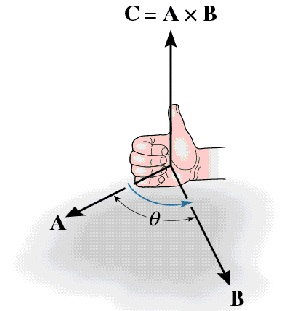
\includegraphics[scale=1]{Gambar/right-hand-rule}
\caption[Right-hand rule dalam \textit{cross product} vektor]{Right-hand rule dalam \textit{cross product} vektor} 
\label{fig:right-hand-rule}
\end{figure}\\
\textit{Quaternion} memiliki persamaan umum yang memiliki empat bilangan riil atau skalar. Persamaan tersebut adalah 
\[
	q = q_0 + i q_1 + j q_2 + k q_3
\]\cite{kuipers:1999}
Sama seperti pada bilangan kompleks, \textit{quaternion} juga memiliki konjugasi kompleksnya. Berikut adalah konjugasi kompleks \textit{quaternion}
\[
	q = q_0 - i q_1 - j q_2 - k q_3
\]





